% Front matter of the extension paper: cover, contents, abstract, relation to
% the thesis, reproducibility statement.

%---------------------------------------------------------------- cover page
\begin{titlepage}
\centering
\vspace*{1.2cm}
{\Huge\scshape S\,G\,R\ \ A*\par}
\vspace{0.3cm}
{\Large\scshape Extension\par}
\vspace{0.6cm}
{\LARGE Seeing Sagittarius A*:\\[2pt]
true colour, moving observers and orbiting hot spots\par}
\vspace{0.8cm}
{\large An extension of the first-principles relativistic simulator of the\\
Galactic-Centre black hole\par}
\vspace{1.2cm}
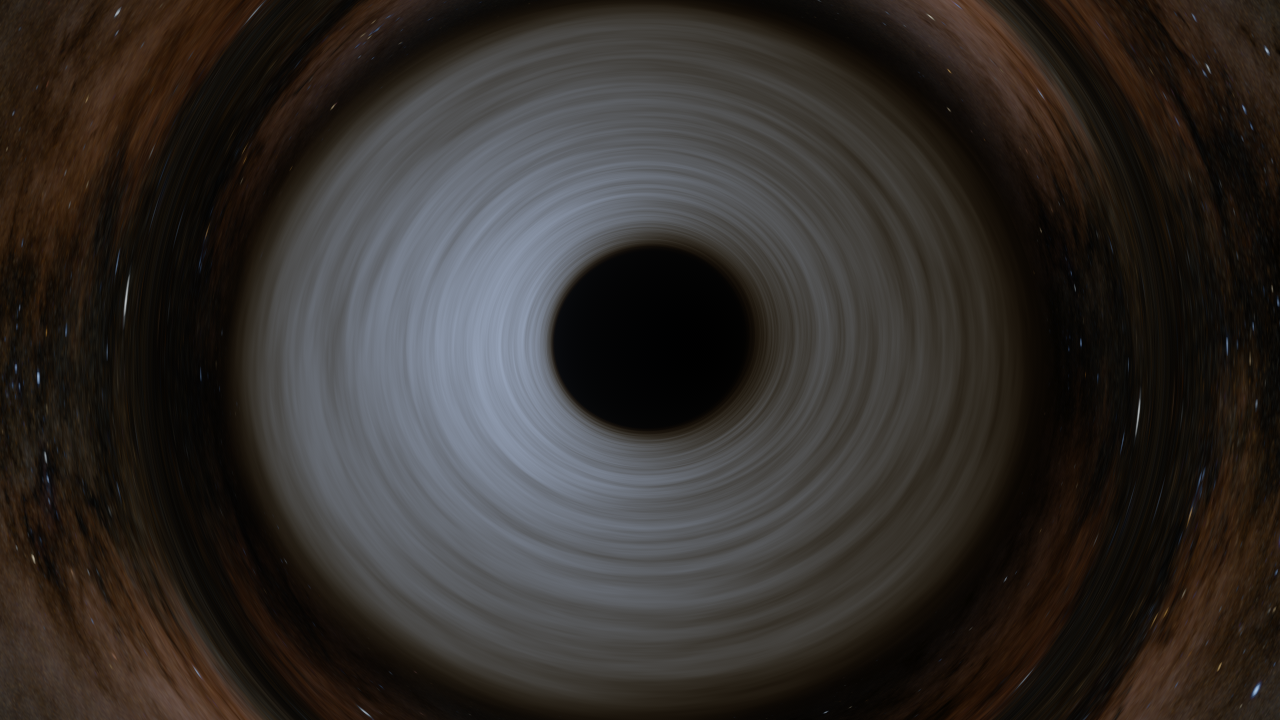
\includegraphics[width=0.82\textwidth]{figures/x_preset1_earth.png}
\vfill
{\large C.~Excelsis\par}
\vspace{0.3cm}
{\large Independent research report --- companion to the thesis\par}
\vspace{0.3cm}
{\large \today\par}
\end{titlepage}

%---------------------------------------------------------------- contents
\pagenumbering{roman}
\tableofcontents
\listoffigures
\listoftables
\cleardoublepage

%---------------------------------------------------------------- abstract
\chapter*{Abstract}
\addcontentsline{toc}{chapter}{Abstract}

This report extends the Sgr~A* simulator of the accompanying thesis from
measuring the black hole to \emph{seeing} it: every image is now rendered as
a camera would record it, from any observer's eyes, with time-dependent
sources --- and every new number is again produced by tested code. All
scenes use one spacetime, Sgr~A* with $\astar = 0.94$ and the GRAVITY mass and
distance.

(i)~\emph{Spectral rendering.} A redshifted blackbody is a blackbody at
$gT$, so one Planck--CIE lookup carries Doppler colour and beaming. The live
GPU renderer now reproduces the fp64 CPU reference pixel for pixel (median
luminance difference \XLiveDlnYMed, 95th percentile \XLiveDlnYPninetyfive\,\%;
Doppler contrast within \XLiveBeamErr\,\%). A thin disk fed at Sgr~A*'s
measured accretion rate would peak at $\XTpeakLow$--$\XTpeakHigh$\,K and shine
$\XLumFactorLow$--$\XLumFactorHigh$ times brighter than Sgr~A* actually does
--- a quantitative reason its real accretion flow cannot be a thin disk. A
camera's Doppler contrast differs from the bolometric $g^4$ law: stronger
below $\approx\XContrastCrossT$\,K, weaker above.
(ii)~\emph{A horizon-penetrating integrator.} Cartesian Kerr--Schild
Hamiltonian geodesics with an analytic gradient replace the Boyer--Lindquist
live kernel, removing its polar seam.
(iii)~\emph{Observers.} Static, orbiting, free-falling and hovering
observers see the aberrated, Doppler-shifted sky predicted by their Lorentz-
boosted tetrads; the Schwarzschild shadow edges match Synge's formula plus
special-relativistic aberration to $\XAberrationCheck$, and the live renderer
matches the fp64 reference to $\XObsGpuMaxPx$ pixel. The comparison exposed,
and fixed, a step-budget defect that had widened the prograde edge of the
high-spin shadow by $\XLegacyBudgetPx$ pixels.
(iv)~\emph{Flares.} A Gaussian hot spot on the orbit GRAVITY fitted to the
2018 near-infrared flares ($R = 7\,M$, $i \approx 160\degr$), traced with
slow light, has a period of $\XFlGraPeriod$\,min (observed $40\pm8$\,min) and
moves clockwise as observed, but its centroid travels only $\XFlGraChord\,\muas$
in 30\,minutes against the observed $\sim$120\,$\muas$ --- reproducing,
independently, the tension GRAVITY reported between flare periods and loop
sizes. Each flash returns as a photon-ring echo $\XFlGraEchoMinMin$--$\XFlGraEchoMaxMin$
minutes later.
(v)~\emph{The hot flow at 230\,GHz.} A semi-analytic radiatively
inefficient flow, normalised to the EHT's $\XRiafTarget$\,Jy and traced with
thermal-synchrotron radiative transfer, puts its light in a Doppler-boosted
crescent inside the photon ring. Its ring, $\XRiafDraw\,\muas$, and its
first visibility minimum, $\XRiafNullMin\,{\rm G}\lambda$, are smaller than
the EHT's $51.8\,\muas$ and $3.0\,{\rm G}\lambda$: the emission must sit
further out, for instance in cooler electrons. Transported to the camera
with the Walker--Penrose constant, its polarisation shows a radial pattern
for a toroidal field, which the EHT excludes. Only a vertical, poloidal field
produces the observed spiral ($\angle\beta_2 = \XPolVerArgCw\degr$ for
clockwise rotation).

(vi)~\emph{Forecasts for S2.} Fisher forecasts from the thesis' own forward
model, checked against its profile likelihood, show that the no-hair
constraint tightens much faster than the thesis' $1/\sqrt{N}$ extrapolation.
Ten more orbits of existing quality would give $\sigma(\epsq) = \XFcTenFisher$,
not $\XFcTenThesis$, because $\epsq$ acts through a secular precession. An
extended mass at GRAVITY's present bound, left out of the fit, becomes a
$\XFcBiasEpsThirtyTwo\sigma$ false no-hair signal after 32 years of
GRAVITY-quality data, invisible in the fit's $\chi^2$. Fitting it jointly
costs only a factor $\XFcInflThirtyTwo$. Frame dragging in S2's orbit needs
$\XFcLtThreeTen$ years of $10\,\muas$ astrometry for a $3\sigma$ detection.
(vii)~\emph{Falling into Sgr~A*.} A timelike geodesic in the ingoing
Kerr--Schild chart carries the camera through the event horizon, with its
conserved quantities kept to $\XIfMaxdQ$. From $\XIfRzero\,M$, the faller
reaches the horizon after $\XIfTauHorMin$ minutes of proper time, and the
inner horizon, where the model stops, $\XIfTauInsideSec$\,s later. The tidal
stretch across a 2\,m body is $\XIfStretchHor$\,m\,s$^{-2}$ at the horizon.
Ahead, the sky skimming the dark region is blueshifted up to
$\XIfEdgeZeroNineMax$-fold. The live view matches the double-precision
tracer to $\XIfGpuMaxPx$ pixel, inside the horizon as well as outside.

An appendix applies the renderer to an exotic spacetime that is \emph{not}
Sgr~A*, the traversable wormhole of \emph{Interstellar}, as a test of its
generality.

%---------------------------------------------------------------- relation
\chapter*{Relation to the thesis}
\addcontentsline{toc}{chapter}{Relation to the thesis}

This is a companion report, deliberately kept separate from the thesis. It
reuses the thesis' physics library, validation conventions and calibration
(e.g.\ one gravitational radius subtends $\UasPerM\,\muas$ and one unit of
geometric time is \XMinPerM\ minutes at the GRAVITY mass and distance), and it
cites the thesis' chapters rather than repeating them. Two thesis results are
prerequisites:

\begin{itemize}
\item the image-handedness correction (thesis Appendix ``Image handedness:
an error found and corrected''): every camera here traces the photon it
\emph{receives}; images are not mirrored;
\item the validated Carter/Mino science path, which remains the reference
against which every new renderer in this report is tested.
\end{itemize}

Display-only processing (exposure, bloom, white balance, tone curve, false
colour) is labelled wherever it appears and never enters a measurement.

%---------------------------------------------------------------- repro
\chapter*{Reproducibility}
\addcontentsline{toc}{chapter}{Reproducibility}

Every number in this report is a macro in \texttt{numbers\_ext.tex}. The
macros are written by the script \texttt{make\_numbers\_ext.py} (in
\texttt{scripts/}) from the JSON and CSV outputs of the tools listed in
Appendix~\ref{app:xrepro}. Every figure is generated by
\texttt{make\_figures\_ext.py} or rendered by a documented engine command.
\texttt{make reproduce-ext} regenerates all of them.

\cleardoublepage
\pagenumbering{arabic}
